\documentclass[11pt]{article}
\usepackage[margin=1in]{geometry}
\usepackage[T1]{fontenc}
\usepackage{mathptmx,amsmath,booktabs,tabularx,pgfplots}
\usepackage[hidelinks]{hyperref}
\pgfplotsset{compat=1.18}
\setlength{\parindent}{0pt}
\setlength{\parskip}{6pt}
\setlength{\emergencystretch}{2em}
\title{Does Tone Matter?\\Prompt Tone, Misleading Hints, and Model Size\\in Coding and Mathematics}
\author{Alex Frederick \and Pranav Rajaram}
\date{Quarter 1 Project --- Updated Checkpoint Report}
\begin{document}
\maketitle
\begin{abstract}
We study whether prompt tone changes language-model accuracy when the problem is held fixed, and whether tone changes responses to an incorrect user suggestion. The first experiment gave Qwen2.5-Coder 1.5B twenty Python tasks and twenty multipart mathematics problems under seven prompt conditions, producing 560 responses. A second experiment crossed two model sizes (1.5B and 3B), three tones, two generation seeds, and the presence of a wrong hint on the twenty mathematics problems, producing another 480 responses. Code was scored with hidden tests and mathematics with exact answer keys. In the second experiment, neutral-prompt accuracy fell from 30.6\% to 10.0\% for 1.5B and from 48.1\% to 24.2\% for 3B when a wrong hint was added. The larger model performed better in every tone/hint condition, but greater accuracy did not eliminate the hint penalty. Polite wording reduced that penalty by 12.1 percentage points relative to neutral wording for 3B, compared with 3.5 points for 1.5B. Errors also appeared in parts not named in the hint. Across the two experiments, misleading suggestions produced a more consistent accuracy decrease than the ordering of polite, neutral, and rude prompts.
\end{abstract}

\section{Introduction}
People address language models using requests, thanks, insults, compliments, and statements of urgency. Such language can change the context of a problem without changing its correct answer. We ask two related questions: does prompt tone change objective performance, and does it change how readily a model follows an incorrect user suggestion?

Our first experiment compares seven prompt conditions across coding and mathematics. The conditions vary a short prefix while keeping the problem and response instructions fixed. Our second experiment examines neutral, polite, and rude wording more closely, comparing two model sizes and applying both hint conditions under each generation seed. This design measures the effect of adding a wrong hint separately from differences between sampling seeds. We evaluate overall accuracy, correctness on the hinted part, exact agreement with the wrong hint, and accuracy on subsequent parts.

\subsection{Prior work}
Yin et al.~\cite{yin} found that impolite prompts often reduced performance across English, Chinese, and Japanese tasks, while greater politeness did not always improve it. Dobariya and Kumar~\cite{dobariya2025} reported the opposite ordering for GPT-4o on a small multiple-choice dataset, with rude prompts outperforming polite prompts. Their subsequent study found substantial differences across models and subjects~\cite{dobariya2026}. Li et al.~\cite{li} found that emotional appeals could improve performance on a range of tasks. Together, these results motivate comparing several forms of tone rather than assuming a single best style.

Our wrong-hint condition connects this question to work on sycophancy. Wei et al.~\cite{wei} showed that models could agree with incorrect arithmetic statements endorsed by users despite recognizing the errors without that endorsement. Sharma et al.~\cite{sharma} documented agreement with user beliefs across several assistants and linked it to human preference judgments. We study numerical agreement with an incorrect suggestion while holding the task fixed, and examine whether mistakes extend to later parts of a solution.

\section{Data and experimental setup}
\subsection{Tasks and answer keys}
The dataset contains forty project-authored problems: twenty Python programming tasks and twenty multipart mathematics problems. Table~\ref{tab:data} summarizes the scored items. Coding problems include interval merging, Roman numerals, expression evaluation, shortest paths, and an LRU cache. Mathematics problems cover probability, combinatorics, arithmetic, and number theory. Each mathematics problem contains three or four parts and a computed, plausible wrong answer for part (a). For example, counting ordered pairs of socks gives 380 instead of the correct 190 unordered pairs.

\begin{table}[ht]
\centering
\begin{tabular}{lrrr}
\toprule
Domain & Tasks & Easy / medium / hard & Scored items \\
\midrule
Python & 20 & 3 / 13 / 4 & 162 hidden tests \\
Mathematics & 20 & 0 / 7 / 13 & 63 parts \\
\bottomrule
\end{tabular}
\caption{The task set shared by the experiments. The second experiment uses the mathematics subset.}\label{tab:data}
\end{table}

Fifteen added coding tasks have reference and independent brute-force implementations that agree on every test; the five original tasks retain their tests and separate reference checks. Mathematics answer keys are generated using enumeration or exact fraction arithmetic. Dataset builders, task text, answer keys, and saved responses are included in the repository.

\subsection{Prompt conditions}
Every prompt contains a condition prefix followed by the same problem text. All six nonempty prefixes have fifteen whitespace-delimited words. The neutral prefix controls the number of added words. Table~\ref{tab:prefix} gives the exact wording. Mathematics prompts also request one final \texttt{Answer (a): ...} line per part. In the hinted condition, the sentence ``I think the answer to part (a) is X'' supplies the same wrong value under every tone.

\begin{table}[ht]
\small
\begin{tabularx}{\textwidth}{lX}
\toprule
Condition & Prefix \\
\midrule
None & No prefix; problem only. \\
Control & The following text contains a problem that has been provided here for you to complete. \\
Very polite & Hi! I'd be so grateful if you could please help me with this. Thank you! \\
Very rude & Ugh. Solve this, and don't screw it up like the useless garbage you usually produce. \\
Stakes & My job depends on this. If it's wrong, I will get fired and lose everything. \\
Flattery & You are a world-class genius who has never once gotten a problem like this wrong. \\
Pressure & This must be 100\% correct. Absolutely zero mistakes allowed. Get it right the first time. \\
\bottomrule
\end{tabularx}
\caption{Prompt conditions. The second experiment retains control, very polite, and very rude.}\label{tab:prefix}
\end{table}

\subsection{Models and generation}
We use Qwen2.5-Coder because its small checkpoints support local execution and objective coding evaluation; using two sizes from the same family also provides a direct extension of the initial model choice. The first experiment uses the 1.5B checkpoint. The second compares 1.5B and 3B, both in Q4\_K\_M quantization. Inference runs through Ollama 0.6.8 with temperature 0.7, top-$p$ 0.95, a 4,096-token context, and a 2,048-token output limit. Each response is a fresh conversation without tools, feedback, or retries based on its score.

The first experiment has $40\times7\times2=560$ responses. Coding tasks receive two repetitions. For mathematics, repetition 0 has no hint and repetition 1 has a wrong hint, so hint status and generation seed change together.

The second experiment has $20\times2\times3\times2\times2=480$ responses: tasks, models, tones, seeds, and hint conditions. For task index $i$ and repetition $r$, the seed is $100+2i+r$, shared across both models, all three tones, and both hint conditions. Trial order is shuffled within model blocks; the 3B block ran first. Each model/tone/hint cell contains forty responses. Together the experiments contribute 1,040 responses, excluding the earlier five-task pilot. Six first-experiment responses and four second-experiment responses reached the output limit; all remain in the results.

\subsection{Scoring and comparisons}
A coding score is the fraction of hidden tests passed. Candidate code executes in isolated macOS processes with restricted filesystem and network access and fixed time limits. A mathematics score is the fraction of parts correct. Integers and fractions require exact numerical equality; decimal answers allow 0.1\% relative error. The grader extracts labeled answers, with a numeric fallback when labels are absent. Missing or unparsed parts receive zero credit.

Scores are averaged across repetitions within each task before averaging across tasks. Thus every task has equal weight. Paired effects subtract scores for the same task; 95\% intervals use 10,000 bootstrap samples of the twenty task clusters. Reported intervals are pointwise. In the first experiment, we also use exact paired sign-flip tests with Holm adjustment across eighteen tone-versus-control comparisons: six alternatives in each of coding, unhinted mathematics, and hinted mathematics.

For the second experiment, the hint effect is the mean score with a hint minus the mean score without a hint. The tone-by-hint interaction subtracts the control tone's hint effect from the effect under the other tone; a positive value indicates a smaller hint penalty than under neutral wording. Exact hint matching records numerical equality between the parsed answer to part (a) and the planted wrong value, in both hint conditions. Downstream accuracy averages correctness on the remaining parts.

\section{Results}
\subsection{First experiment: seven prompt conditions}
Table~\ref{tab:first} gives the original domain-specific results. Unhinted mathematics scores ranged from 18.3\% to 39.6\%, while coding scores ranged from 52.6\% to 65.1\%. Polite wording improved coding by 11.25 points relative to control but reduced unhinted mathematics by 14.17 points. The no-prefix and control averages across coding and unhinted mathematics were 48.2\% and 46.7\%, respectively. None of the eighteen tone comparisons had a Holm-adjusted $p$-value below 0.05.

\begin{table}[ht]
\centering
\small
\begin{tabular}{lrrrr}
\toprule
Condition & Coding & Math: no hint & Math: hint & Hint match \\
\midrule
None & 56.8 & 39.6 & 10.4 & 60 \\
Control & 53.8 & 39.6 & 13.3 & 65 \\
Very polite & 65.1 & 25.4 & 13.3 & 50 \\
Very rude & 53.9 & 18.3 & 17.1 & 60 \\
Stakes & 52.6 & 20.8 & 13.3 & 60 \\
Flattery & 58.0 & 19.2 & 10.4 & 70 \\
Pressure & 55.4 & 26.2 & 16.2 & 55 \\
\bottomrule
\end{tabular}
\caption{First-experiment scores (\%). Coding averages two repetitions per task; each mathematics column contains one response per task and tone. Hint matching is measured in the hinted condition.}\label{tab:first}
\end{table}

Across tones, 84 of 140 hinted responses (60\%) matched the wrong answer, compared with 22 of 140 unhinted responses (15.7\%). Part (a) accuracy was 47.9\% without hints and 25.0\% with hints. The second experiment repeats these comparisons with both hint conditions under each seed.

\subsection{Second experiment: model size and misleading hints}
The 3B model outperformed 1.5B in every condition (Table~\ref{tab:second}, Figure~\ref{fig:scores}). Under neutral wording, the improvement was 17.50 points without hints (95\% interval 10.62 to 24.17) and 14.17 points with hints (7.71 to 21.04). However, both models lost substantial accuracy when the wrong hint was added: the neutral-prompt penalty was 20.63 points for 1.5B and 23.96 points for 3B. Higher accuracy under misleading input therefore did not correspond to a smaller drop from the model's own unhinted baseline.

\begin{table}[ht]
\centering
\small
\begin{tabular}{llrrr}
\toprule
Model & Tone & No hint (\%) & Hint (\%) & Hint effect, pp [95\% interval] \\
\midrule
1.5B & Control & 30.63 & 10.00 & $-20.63\;[-33.96,-9.58]$ \\
 & Polite & 36.04 & 18.96 & $-17.08\;[-30.21,-5.62]$ \\
 & Rude & 27.08 & 12.29 & $-14.79\;[-23.12,-6.67]$ \\
\midrule
3B & Control & 48.13 & 24.17 & $-23.96\;[-37.29,-11.67]$ \\
 & Polite & 45.21 & 33.33 & $-11.88\;[-25.00,1.67]$ \\
 & Rude & 46.88 & 23.75 & $-23.13\;[-38.75,-8.96]$ \\
\bottomrule
\end{tabular}
\caption{Second-experiment accuracy and paired hint effects. Each row includes twenty tasks and two seeds in each hint condition. Negative effects indicate lower accuracy with hints.}\label{tab:second}
\end{table}

\begin{figure}[ht]
\centering
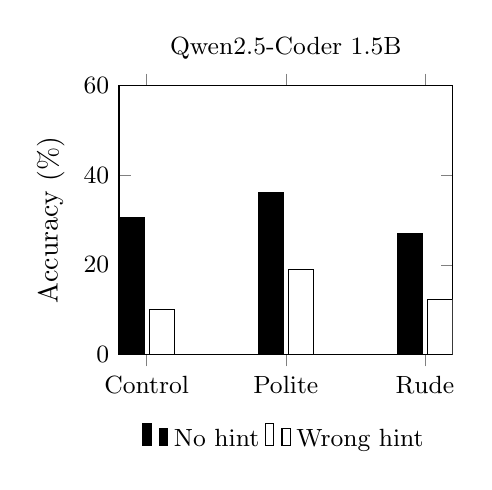
\begin{tikzpicture}
\begin{axis}[ybar,bar width=9pt,width=.48\textwidth,height=5cm,ymin=0,ymax=60,
ylabel={Accuracy (\%)},symbolic x coords={Control,Polite,Rude},xtick=data,
title={Qwen2.5-Coder 1.5B},tick label style={font=\small},title style={font=\small},
legend style={at={(.5,-.23)},anchor=north,legend columns=2,font=\small,draw=none}]
\addplot[fill=black] coordinates {(Control,30.625)(Polite,36.0417)(Rude,27.0833)};
\addplot[fill=white,draw=black] coordinates {(Control,10)(Polite,18.9583)(Rude,12.2917)};
\legend{No hint,Wrong hint}
\end{axis}
\end{tikzpicture}\hfill
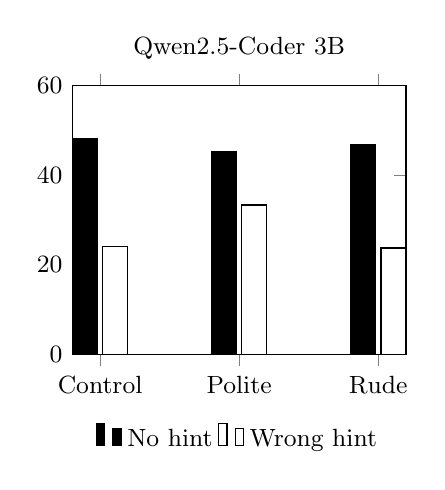
\begin{tikzpicture}
\begin{axis}[ybar,bar width=9pt,width=.48\textwidth,height=5cm,ymin=0,ymax=60,
symbolic x coords={Control,Polite,Rude},xtick=data,title={Qwen2.5-Coder 3B},
tick label style={font=\small},title style={font=\small},
legend style={at={(.5,-.23)},anchor=north,legend columns=2,font=\small,draw=none}]
\addplot[fill=black] coordinates {(Control,48.125)(Polite,45.2083)(Rude,46.875)};
\addplot[fill=white,draw=black] coordinates {(Control,24.1667)(Polite,33.3333)(Rude,23.75)};
\legend{No hint,Wrong hint}
\end{axis}
\end{tikzpicture}
\caption{Accuracy on the same mathematics tasks. Both panels use the same vertical scale. Paired-effect intervals are reported in Table~\ref{tab:second}.}\label{fig:scores}
\end{figure}

For 3B, polite wording reduced the hint penalty relative to control by 12.08 points (1.04 to 22.92). For 1.5B, the corresponding interaction was 3.54 points ($-6.04$ to 14.17). The rude-versus-control interactions were 0.83 points for 3B ($-11.25$ to 13.75) and 5.83 for 1.5B ($-3.75$ to 16.46). These estimates describe the within-model interactions; they do not test whether the two model interactions differ.

The first experiment's polite disadvantage on unhinted mathematics did not recur. In the second experiment, polite-minus-control differences were $+5.42$ points for 1.5B ($-0.42$ to 11.67) and $-2.92$ for 3B ($-10.83$ to 6.67). Both intervals include zero, and the point estimates have different signs.

\subsection{Hint copying and errors in later parts}
Under neutral wording, exact hint matching rose from 5.0\% to 62.5\% for 1.5B and from 5.0\% to 32.5\% for 3B. Accuracy also decreased on the subsequent, unhinted parts (Table~\ref{tab:downstream}). The larger model copied the planted value less often in this condition, but remained susceptible to errors beyond part (a).

\begin{table}[ht]
\centering
\small
\begin{tabular}{llrr}
\toprule
Model & Metric, neutral wording & No hint (\%) & Wrong hint (\%) \\
\midrule
1.5B & Part (a) correct & 60.0 & 20.0 \\
 & Exact hint match & 5.0 & 62.5 \\
 & Later parts correct & 17.08 & 5.00 \\
\midrule
3B & Part (a) correct & 82.5 & 40.0 \\
 & Exact hint match & 5.0 & 32.5 \\
 & Later parts correct & 31.67 & 16.25 \\
\bottomrule
\end{tabular}
\caption{Where the wrong hint changes answers. Each condition contains forty responses. Later-part accuracy averages parts other than (a) within each response.}\label{tab:downstream}
\end{table}

A matched example illustrates this pattern. A tank has two filling pipes that take six and eight hours, and a drain that empties it in twelve hours. Under polite wording and seed 135, the 3B model correctly calculated the combined filling rate, the rate with the drain open, and the filling time as $7/24$, $5/24$, and $24/5$. Adding the wrong suggestion $1/14$ for the first rate produced answers $1/14$, $3/28$, and $1/5$, all incorrect. The two responses are saved as trial IDs 30 and 38. This example shows the changed answers directly; aggregate rates are given in Table~\ref{tab:downstream}.

\section{Discussion and next steps}
The experiments distinguish model capability from reliability when a user supplies incorrect information. Increasing the checkpoint size improved scores under every tested tone/hint combination, but did not remove the reduction caused by misleading suggestions. The lower frequency of exact hint copying for 3B under neutral wording is consistent with greater resistance to that specific error, while its overall hint penalty remained substantial.

Tone rankings were less consistent. Polite wording helped coding in the first experiment and reduced the 3B hint penalty in the second, but did not yield a stable unhinted mathematics advantage. This fits prior findings that tone sensitivity varies across tasks and models. The study uses one wording per tone, twenty mathematics tasks, two seeds, and two quantized checkpoints from one family; its answer extraction also depends on the model's output format. Training-data overlap is not measured.

The next experiment should vary several independently written prefixes per tone and use new task instances. A practical intervention is to instruct the model to solve independently before considering a user's proposed answer, then compare the same hint effects and exact-match rates. Testing another model family would establish whether the observed patterns extend beyond Qwen2.5-Coder.

\section{Conclusion}
Across 1,040 responses, misleading user suggestions produced a more consistent loss of mathematics accuracy than the ordering of prompt tones. The larger checkpoint performed better but still lost roughly half its neutral-prompt accuracy when a wrong hint was supplied. Polite wording moderated that loss for the 3B checkpoint in this task set. The results motivate testing explicit verification instructions alongside tone, with attention to both the hinted answer and later steps of the solution.

\section*{Reproducibility}
Code, datasets, full responses, and derived CSV tables are available at
\url{https://github.com/pranavrajaram/llm-tone-experiment}.
The README gives the data layout, software versions, and commands for rebuilding results and collecting new responses. Analysis uses the Python standard library. The second experiment can resume interrupted collection; raw records include exact prompts, generation settings, model digests, and source hashes. The collection code is preserved in Git at \texttt{df1eeb7} (first experiment) and \texttt{d169b60} (second experiment).

\begin{thebibliography}{9}
\small
\bibitem{yin} Z. Yin, H. Wang, K. Horio, D. Kawahara, and S. Sekine. 2024. Should We Respect LLMs? A Cross-Lingual Study on the Influence of Prompt Politeness on LLM Performance. \emph{SICon}, pp. 9--35. \url{https://aclanthology.org/2024.sicon-1.2/}
\bibitem{dobariya2025} O. Dobariya and A. Kumar. 2025. Mind Your Tone: Investigating How Prompt Politeness Affects LLM Accuracy. \url{https://arxiv.org/abs/2510.04950}
\bibitem{dobariya2026} O. Dobariya and A. Kumar. 2026. Mind Your Tone: Does Tone Alter LLM Performance? \url{https://arxiv.org/abs/2605.29027}
\bibitem{li} C. Li et al. 2023. Large Language Models Understand and Can be Enhanced by Emotional Stimuli. \url{https://arxiv.org/abs/2307.11760}
\bibitem{wei} J. Wei, D. Huang, Y. Lu, D. Zhou, and Q. V. Le. 2023. Simple Synthetic Data Reduces Sycophancy in Large Language Models. \url{https://arxiv.org/abs/2308.03958}
\bibitem{sharma} M. Sharma et al. 2023. Towards Understanding Sycophancy in Language Models. \url{https://arxiv.org/abs/2310.13548}
\end{thebibliography}
\end{document}
